\documentclass[/home/jesse/Analysis/FemtoAnalysis/AnalysisNotes/AnalysisNoteJBuxton.tex]{subfiles}
\begin{document}

\subsection{Pair Selection}
\label{PairSelection}

The femtoscopic analysis of two-particle correlation functions relies on the proper formation of particle pairs.
As such, it is important to obtain true particle pairs in the analysis.  
In particular, contamination from pairs constructed with split or merged tracks, and pairs sharing daughters, can introduce artificial signals into the correlation function, obscuring the actual physics.  
In an effort to remove contamination, we impose two main pair cuts: a shared daughter cut, and an average separation cut.  

The purpose of the shared daughter cut is to ensure the first particle in the pair is unique from the second.  
For pairs formed of two V0s (e.g. \LamKs), this cut is implemented by removing all pairs which share a daughter.
For example, in the \LamKs analysis, if the \Lam and \Ks in a potential pair claim the same $\pi^{-}$ daughter, the pair is excluded from the analysis.  
For a pair formed of a single V0 and a charged track (e.g. \LamKpm), the cut removes all pairs in which the charged track is also claimed as a daughter of the V0.  
This mistake could only occur if, for instance, either a \Kpm is misidentified as a $\pi$ or p and used in the V0 reconstruction, or a $\pi$ or p is misidentified as a \Kpm in the \Kpm selection.
In the case of a pair formed from a charged $\Xi$ and a charged track (e.g. $\Xi^{-}$\Kpm), the cut removes all pairs in which the charged track is also claimed as a daughter of the $\Xi$, be it the bachelor-$\pi$ daughter directly, or a daughter of the \Lam daughter (a granddaughter of the $\Xi$). 
In the $\Xi^{-}$\Kpm analysis, as in the \LamKpm case, this could only occur if there was misidentification of a \Kpm as a $\pi$ or p, or vice versa.

The purpose of the average separation cut is to remove splitting and merging effects, and it is employed in the following way.  
To calculate the average separation between two tracks, the spatial separation is determined at several points throughout the TPC (every 20 cm radially from 85 cm to 245 cm), and the results averaged.
For that \LamKs analysis, which involves two V0 particles, a minimum average separation cut of 6 cm between the like-charge daughters in the pairs was imposed (for example, between the p daughter of the \Lam and the $\pi^{+}$ daughter of the \Ks).
For the \LamKpm analyses, a minimum average separation cut of 8 cm was enforced between the \Kpm and the \Lam daughter sharing the same charge (for example, in the \LamKchP analysis, between the p daughter of the \Lam and the \KchP).
Finally, for the $\Xi^{-}$\Kpm analysis, a minimum average separation cut of 8 cm was enforced between any daughter of the $\Xi$ sharing the same charge as the \Kpm in the pair (for example, the the $\Xi^{-}$\KchM analysis, between the $\pi^{-}$ granddaughter which decayed from the \Lam daughter and the \KchM, and between the bachelor-$\pi^{-}$ daughter and the \KchM).

The motivation for the values used in these cuts can be see in Figures \ref{fig:AvgSepLamK0}, \ref{fig:AvgSepLamKch}, and \ref{fig:AvgSepXiKch}, in which average separation correlation functions are presented.
The average separation correlation functions are formed just as for our relative-momentum correlation functions, but we instead bin in average separation.
Looking at these average separation correlation functions for like-charge tracks, at lowest average separation we see an enhancement due to track splitting, followed by (at slightly higher average separation) a suppression due to track merging.
When the average separation correlation function stabilizes to unity, these effects are no longer abundant, and we choose our cut value.
Splitting and merging effects between oppositely charged tracks was found to be negligible, therefore no cuts on unlike-charge tracks were imposed. To summarize:


\begin{enumerate}
 \item[] Average Separation Cuts ($\overline{\Delta\mathbf{r}}$)
 \begin{enumerate}
  \item \LamKs Analyses
  \begin{itemize}
   \item $\overline{\Delta\mathbf{r}} >$ 6.0 cm for like-charge sign daughters
   \item No cut for unlike-charge daughters
  \end{itemize}
  \item \LamKpm Analyses
  \begin{itemize}
   \item $\overline{\Delta\mathbf{r}}$ $>$ 8.0 cm for daughter of \LamALam sharing charge sign of \Kpm
   \item No cut for unlike-charge
  \end{itemize}
  \item \XiKpm Analyses
  \begin{itemize}
   \item $\overline{\Delta\mathbf{r}}$ $>$ 8.0 cm for any daughter of $\Xi$ sharing charge sign of \Kpm
   \item No cut for unlike-charge
  \end{itemize}  
 \end{enumerate}
\end{enumerate}


\begin{figure}[h]
  \centering
  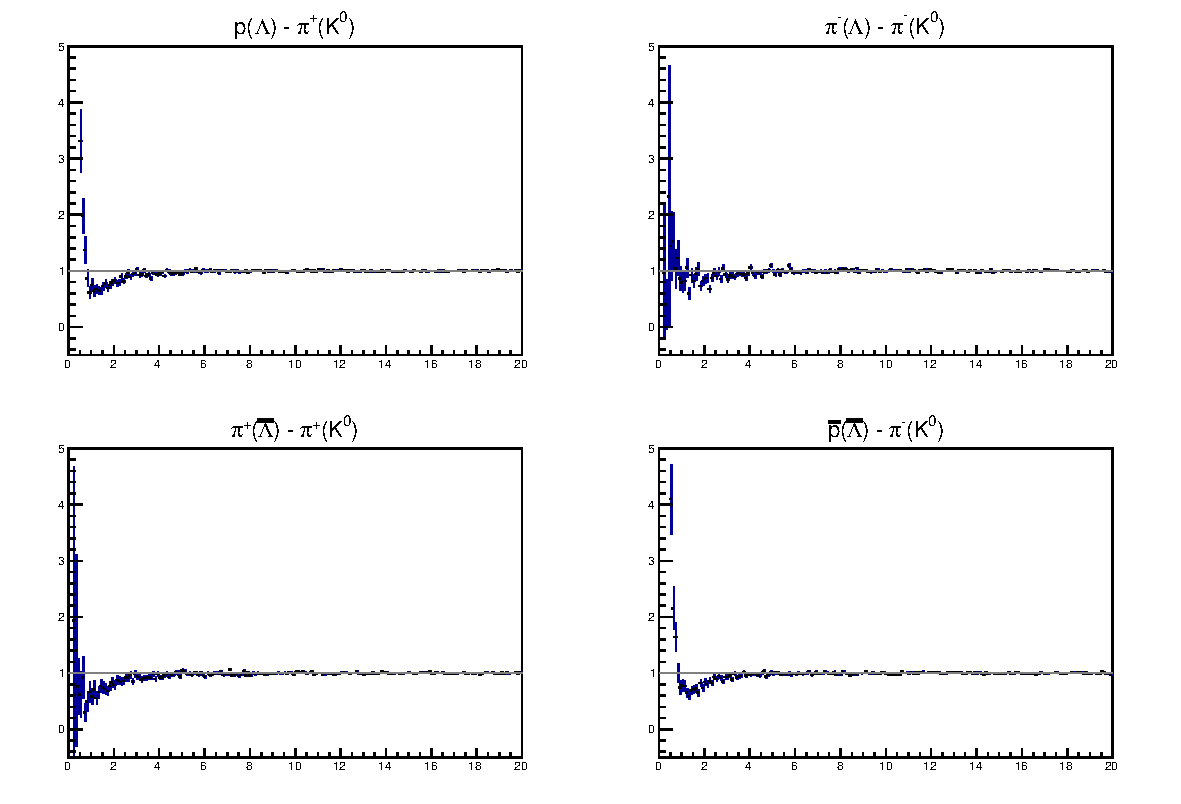
\includegraphics[width=0.8\textwidth]{3_DataSelection/Figures/AvgSepCFs_LamK0.pdf}
  \caption[Avgerage Separation of \LamALam and \Ks Daughters]{Average separation (cm) correlation functions of \LamALam and \Ks Daughters.  Only like-sign daughter pairs are shown (the distributions for unlike-signs were found to be flat).  The title of each subfigure shows the daughter pair, as well as the mother of each daughter (in ``()"),  ex. top left is p from \Lam with $\pi^{+}$ from \Ks.}
  \label{fig:AvgSepLamK0}
\end{figure}

\begin{figure}[h]
  \centering
  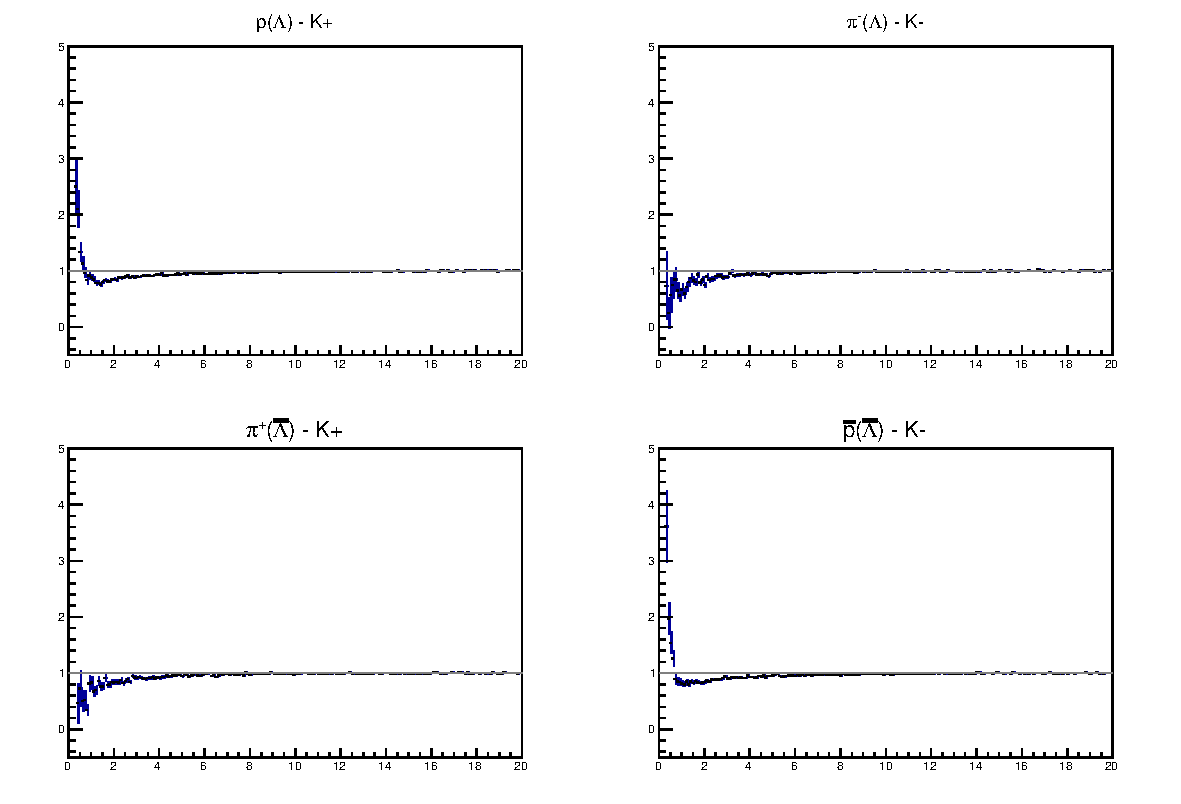
\includegraphics[width=0.8\textwidth]{3_DataSelection/Figures/AvgSepCFs_LamKch.pdf}
  \caption[Avgerage Separation of \LamALam Daughter and \Kpm]{Avgerage separation (cm) correlation functions of \LamALam Daughter and \Kpm.  Only like-sign pairs are shown (unlike-signs were flat).  In the subfigure titles, the particles in ``()" represent the mothers, ex. top left is p from \Lam with \KchP.}
  \label{fig:AvgSepLamKch}
\end{figure}



\begin{figure}[h]
  \centering
  %%----start of first subfigure---  
  \subfloat[$\Xi^{-}$\KchP]{
    \label{fig:AvgSepXiKch:a}
    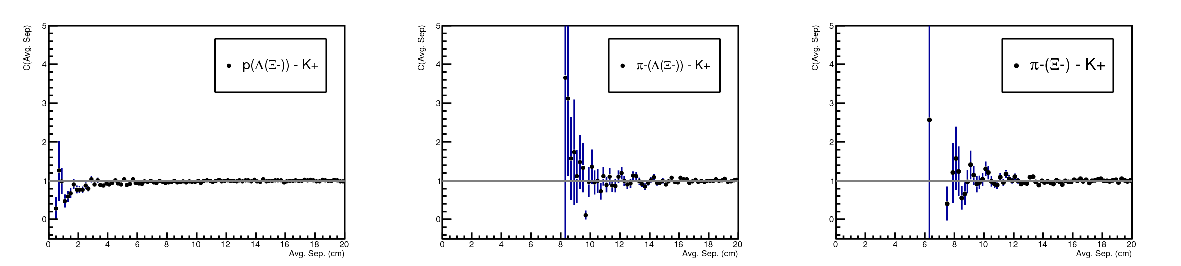
\includegraphics[width=0.99\textwidth]{3_DataSelection/Figures/cXicKchAvgSepCfs_XiKchP.pdf}}\\
  %%----start of second subfigure---
  \subfloat[$\bar{\Xi}^{+}$\KchM]{
    \label{fig:AvgSepXiKch:b}
    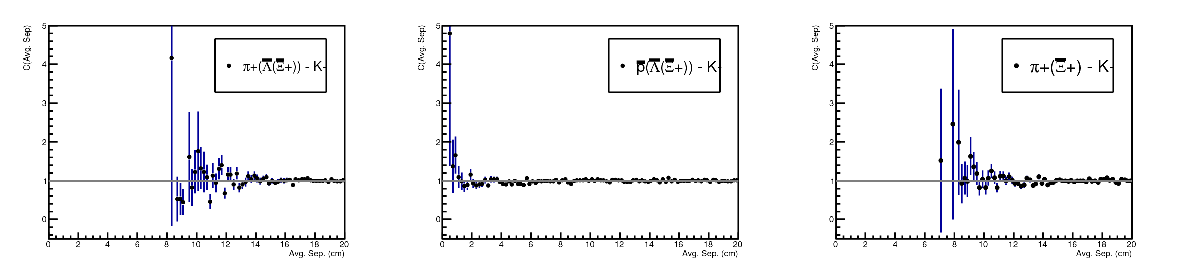
\includegraphics[width=0.99\textwidth]{3_DataSelection/Figures/cXicKchAvgSepCfs_AXiKchM.pdf}}\\
      %%----start of third subfigure---  
  \subfloat[$\Xi^{-}$\KchM]{
    \label{fig:AvgSepXiKch:c}
    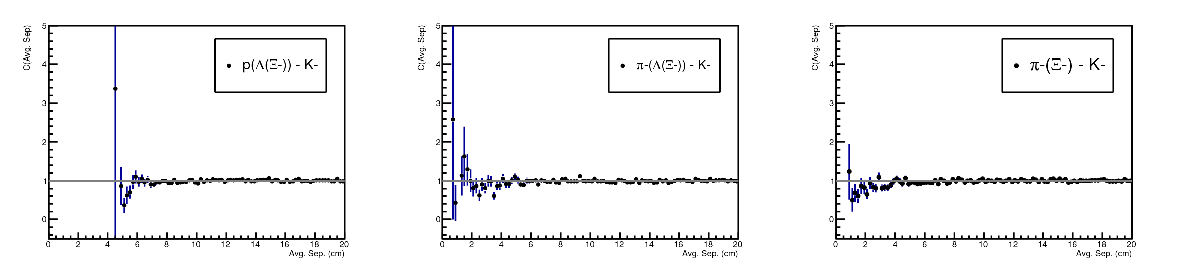
\includegraphics[width=0.99\textwidth]{3_DataSelection/Figures/cXicKchAvgSepCfs_XiKchM.pdf}}\\
  %%----start of fourth subfigure---
  \subfloat[$\bar{\Xi}^{+}$\KchP]{
    \label{fig:AvgSepXiKch:d}
    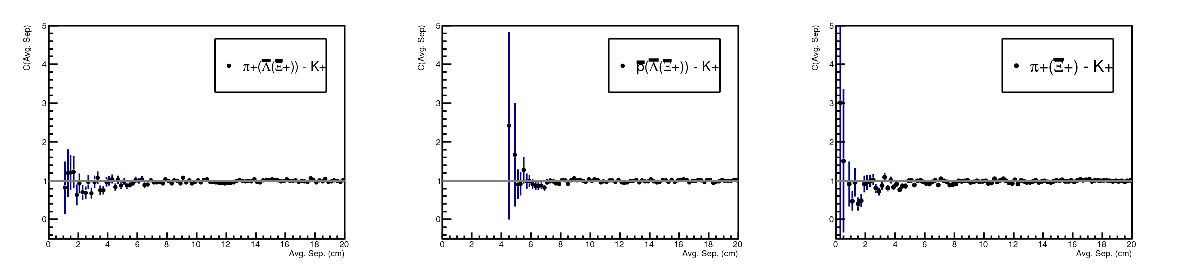
\includegraphics[width=0.99\textwidth]{3_DataSelection/Figures/cXicKchAvgSepCfs_AXiKchP.pdf}}
  %%----overall caption----
  \caption[Avgerage Separation of $\Xi$ Daughters and \Kpm]{Avgerage separation (cm) correlation functions of $\Xi$ Daughter and \Kpm.  In the subfigure titles, the particles in ``()" represent the mothers, ex. top left is p from \Lam from $\Xi^{-}$ with \KchP.}
  \label{fig:AvgSepXiKch}
\end{figure}

\clearpage

\end{document}